\documentclass[11pt,a4paper]{beamer}
\usetheme{Warsaw}
\usecolortheme{beetle}
%\usecolortheme{structure}
\usepackage[MeX]{polski}
\usepackage[utf8]{inputenc}
\usepackage[polish]{babel}
\usepackage{amsmath}
\usepackage{amsfonts}
\setlength{\parindent}{0pt}
\setlength{\parskip}{1ex}
\usepackage{amssymb}
\usepackage{graphicx}
\usepackage{hyperref}

\renewcommand{\qedsymbol}{$\square$}
\newenvironment{dowod}{{\bf Dowód.}}{\hfill\rule[0.025cm]{0.21cm}{0.21cm}}
\usepackage{subfig}
\newtheorem{tw}{Twierdzenie}
\newtheorem{fakt}{Fakt}
\newtheorem{lemat}{Lemat}
\newtheorem{wn}{Wniosek}
\newtheorem{wa}{Ważne}

\title{Równoległy algorytm mrówkowy}
\subtitle{dla jednomaszynowego problemu szeregowania zadań}
\author{Piotr Gródek \and Tomasz Pawlak}
\institute
{
Instytut Informatyki\\
Uniwersytet Wrocławski
}
\begin{document}

\frame{\titlepage}

\section{Wstęp}
\subsection{Opis problemu}

\begin{frame}
\frametitle{Opis problemu}
\begin{itemize}
\item dany jest zbiór \textit{n} ponumerowanych zadań $N = \{1,2,\cdots,n\}$, które należy wykonać bez zatrzymywania na jednej maszynie,   
\item maszyna wykonuje co najwyżej jedno zadanie, 
\item każde zadanie $t_i$ jest opisane przez wartości $p_i, w_i, d_i$:
\begin{itemize}
\item $p_i$ - czas wykonania zadania,
\item $w_i$ - waga funkcji kosztów,
\item $d_i$ - termin wykonania zadania (linia krytyczna).
\end{itemize} 
\item oznaczając prze $C_{i}$ termin zakończenia zadania $i$ wprowadzamy opóźnienie zdefiniowane jako: $$T_{i} = max \{ 0, C_{i} - d_{i} \}$$
\end{itemize} 
\begin{block}{Cel:}
{\color{blue}Szukamy permutacji zadań $\pi$, która minimalizuje wartość $Y(\pi) = \sum w_{\pi(i)} T_{\pi(i)}$}.
\end{block}
\end{frame}

\subsection{Algorytm mrówkowy}
\begin{frame}
\begin{figure}
 \centering
  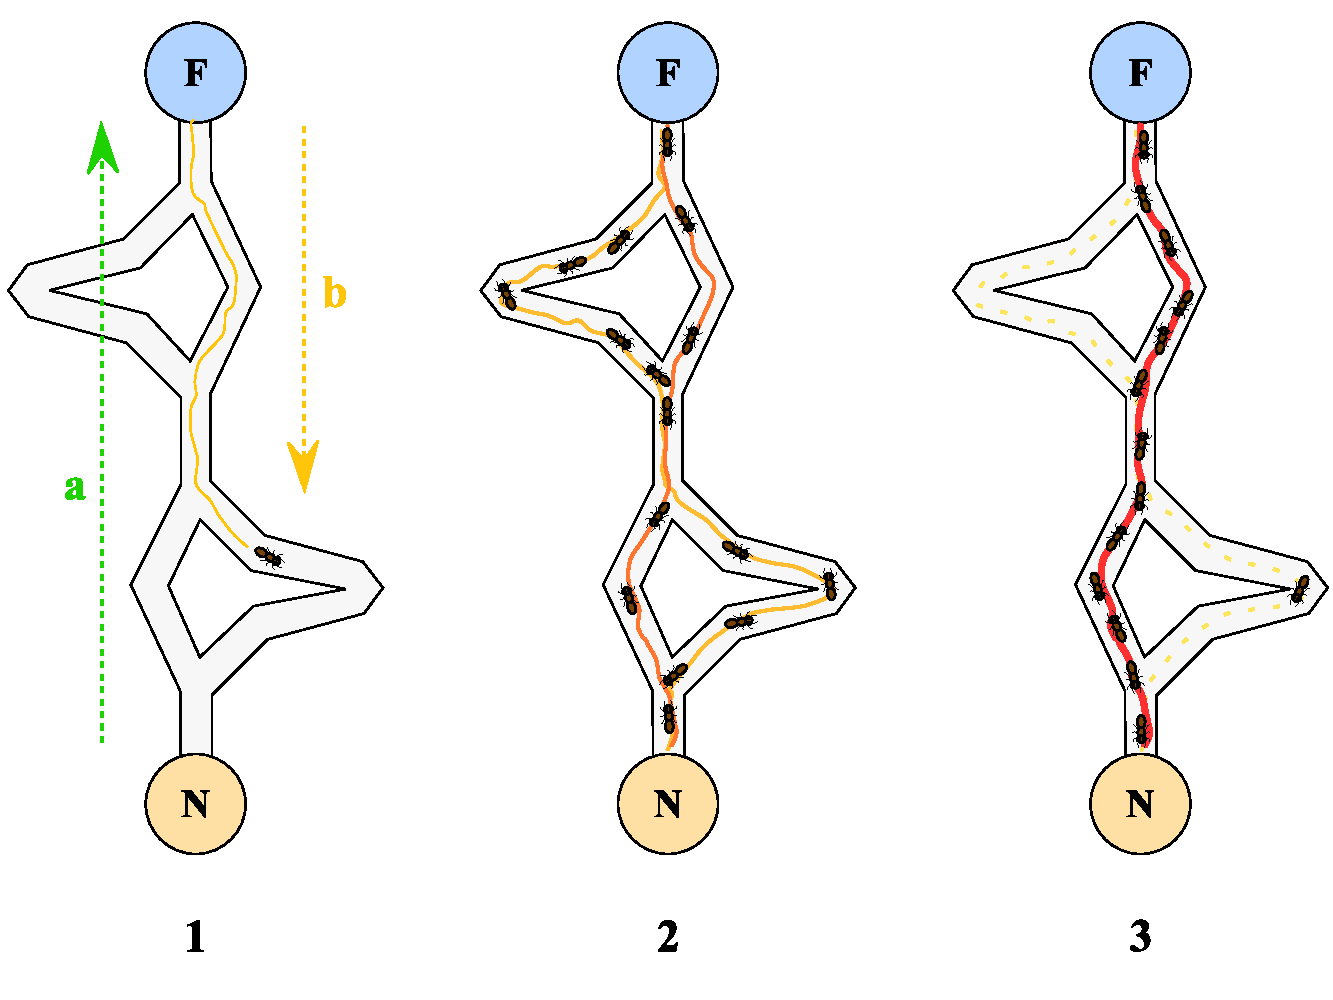
\includegraphics[width=\textwidth]{aco}
  \caption {Idea algorytmu mrówkowego}
\end{figure}
\end{frame}

\subsection{Równoległy algorytm mrówkowy}
\begin{frame}
Najpierw kilka obserwacji:
\begin{itemize}
\item możliwe drogi to wszystkie permutacje zadań
\item liczba feromonu rośnie wraz ze spadkiem wartości $Y(\pi)$
\item mrówka wydaje się idealnym kandydatem na osobny wątek
\end{itemize}
Z tych obserwacji wynika, że:
\begin{itemize}
\item mrówka musi pamiętać które zadania musi jeszcze wykonać - będziemy pamiętać listę zadań do wykonania,
\item będziemy mieć dwuwymiarową tablicę feromonów, gdzie pod indeksem $[i,j]$ będzie liczba feromonu związane z wyborem $j$-tego zadania na miejscu $i$, przy czym jego ilość zostawiona przez mrówkę jest postaci $\frac{1}{Y(\pi)}$,
\item jeśli każda mrówka byłaby osobnym wątkiem to rośnie koszt synchronizacji oraz mamy mniejszy rozrzut badanych ścieżek czyli rośnie prawdopodobieństwo wpadnięcia w lokalne minimum.
\end{itemize}
\end{frame}

\begin{frame}
Nasz algorytm polega na tym, że:
\begin{itemize}
\item tworzymy równoległe \textbf{mrowiska}, które w każdej iteracji wysyłają zadaną liczbę \textit{niezależnych} mrówek (które też są osobnymi wątkami),
\item każde mrowisko pamięta najlepsze osiągnięte wyniki,
\item raz na jakiś czas tworzony jest na tej podstawie ranking mrowisk oraz zostają wymieszane tablice feromonów (najlepsze z najgorszymi).
\end{itemize}

Dodatkowo chcemy mieć graficzny interfejs użytkownika i graficzny podgląd rozkładu feromonów co wymaga uruchomienia kontrolera mrowisk jako osobny wątek i dodatkową synchronizację.

Program został napisany w języku C\# przy użyciu mechanizmów programowania wielowątkowego z platformy .NET 4.0.
\end{frame}

\begin{frame}
\frametitle{Algorytm}
\begin{enumerate}
\item Stwórz $n$ mrowisk jako osobne wątki
\item Dopóki nie przerwano obliczeń:

\begin{enumerate}
\item W każdym mrowisku powtórz $i$ razy:

\begin{enumerate}
	\item Wygeneruj $k$ mrówek
	\item Dla każdej mrówki znajdź ścieżkę na podstawie intensywności feromonu oraz ew. heurystyki
	\item Uaktualnij feromony
\end{enumerate}

\item Posortuj mrowiska względem znalezionych ścieżek
\item Zapamiętaj najlepszą ścieżkę
\item Wymieszaj feromony z zadanymi współczynnikami tak, że najlepszy miesza się z najgorszym itd.
\end{enumerate}
\item Zwróć najlepszą ścieżkę.
\end{enumerate}
\end{frame}

\section{Prezentacja programu}
\begin{frame}[c]
\begin{center}
Czas na prezentację programu :)
\end{center}
\end{frame}


\section{Zakończenie}
\subsection{Wyniki obliczeń i ich analiza}
\begin{frame}
Dane testowe pochodzą ze \href{http://people.brunel.ac.uk/~mastjjb/jeb/orlib/wtinfo.html}{\color{blue}\underline{strony J E Beasley}}.\\

Zaprezentujemy teraz wyniki testów dla przykładowej grupy instancji naszego problemu.

Poza wynikami obliczeń porównaliśmy również wydajność dla różnych konfiguracji programu.
\end{frame}

\subsection{Zakończenie}
\begin{frame}
\begin{center}
Dziękujemy za uwagę.
\end{center}
\end{frame}

\end{document}